\section{Analysis Strategy}
\label{sec:Analysis-Strategy}

At the start a given cut on the Random Forrest Classifier is being made on the reconstructed events (measurement and simulation).
Only events that have a confidence of $\geq 0.8$ as are being selected for further analysis steps.
As well only events with an angular distance to the position of the source of $\theta^2 \leq \num{0.025}$ are being used.

After selecting the data a theta-squared plot is made and the detector significance is being calculated.
The next step is creating the migration matrix of the random forrest regressor with the estimated and true gamma energies in an
energy range from $\SI{500}{\giga\electronvolt}$ to $\SI{15}{\tera\electronvolt}$.

After unfolding the data with the naive SVD and with the Poisson-likelihood method, the results are being compared with the results of HERA and MAGIC

\section{Analysis}

\subsection{Theta-Squared Plot and Detector Significance}
After selecting the data as described in chapter \ref{sec:Analysis-Strategy} the theta-squared plot for on and off-events are being displayed.
Additionally a cut-off point has been found to determine at what values of $\theta^2$ a good difference between on and off-events exists.
The plot as well as the cut off is shown in figure \ref{fig:tsquared}.

\begin{figure}[H]
  \centering
  \includegraphics[width=0.8\textwidth]{plots/On_Off.pdf}
  \caption{Theta-squared plot for on-region and off-region data.}
  \label{fig:tsquared}
\end{figure}

It shows that the off-events are distributed evenly across all values of $\theta^2$.
The on-events show a good difference before the cut off point.
The detector significance for this data set has a value of
\begin{equation}
  S = 26.27587\,.
\end{equation}

\subsection{Migration Matrix and Unfolding}
The estimated values \texttt{gamma\_energy\_prediction} from the given data \texttt{gamma\_test\_dl3\.hdf5}
sample and the true-values \texttt{corsika\_event\_header\_total\_energy} are being used to calculate the migration matrix.
The chosen bins range from $\SI{500}{\giga\electronvolt}$ to $\SI{15}{\tera\electronvolt}$ on a logarithmic scale since inverse problems are often better conditioned when there are more bins in the measured parameter than in the unfolded parameter.
To take events into account that have a higher energy than the upper threshold an additional bin at $\SI{50}{\tera\electronvolt}$  is created.
The migration matrix is shown in figure \ref{fig:matrix}
It is shown that the true values and the estimated values are highly correlated.

\begin{figure}[H]
  \centering
  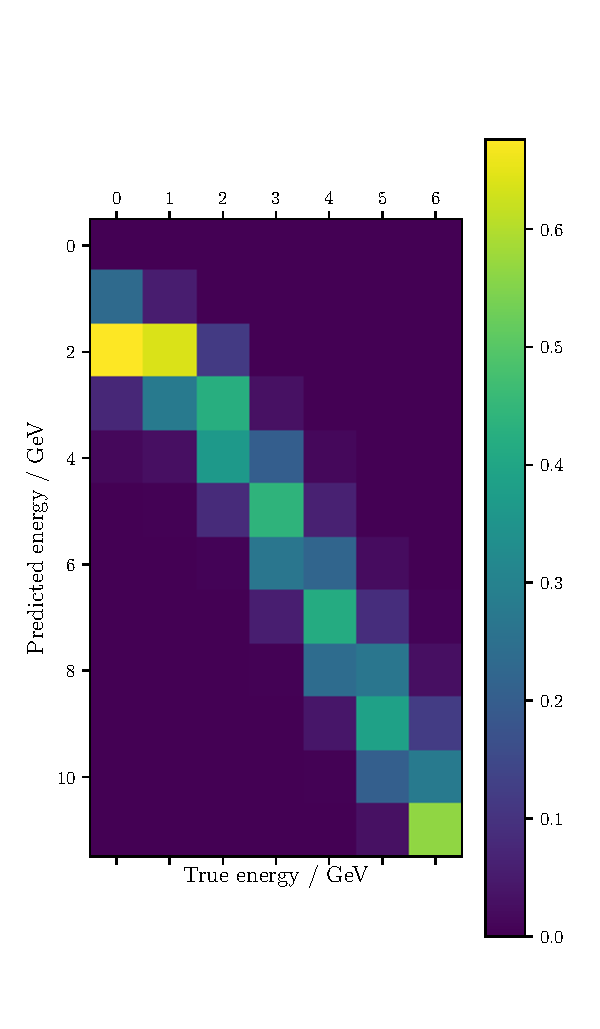
\includegraphics[width=0.5\textwidth]{plots/Matrix.pdf}
  \caption{The migration matrix of the random-forest regressor.}
  \label{fig:matrix}
\end{figure}

\subsection{Naive SVD Unfolding}
The background is taken from off-events and the estimated gamma-events are taken from the on-regions.
The pseudoinverse matrix and the unfolded energies as shown in figure \ref{fig:NSVD} were calculated with \texttt{scipy} and \texttt{uncertainties}.

\begin{figure}[H]
  \centering
  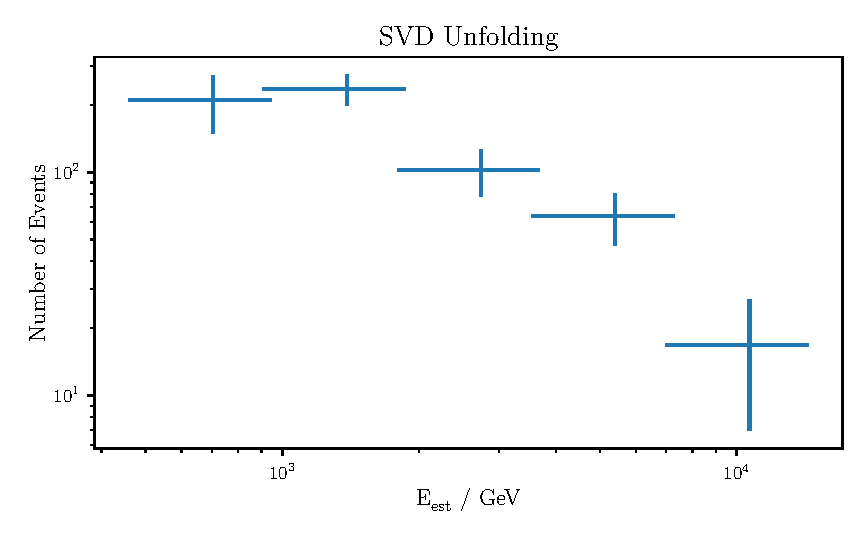
\includegraphics[width=0.8\textwidth]{plots/NSVD.pdf}
  \caption{Unfolded energies with naive SVD.}
  \label{fig:NSVD}
\end{figure}

This method of naive SVD unfolding results to
\begin{align}
\hat{\symbf{f}} &=
\begin{pmatrix}
     210.21 \pm 60.88 \\
     235.61 \pm 36.74 \\
     102.47 \pm 24.21 \\
     63.46 \pm 16.53 \\
     16.90 \pm 9.94 \\
\end{pmatrix}
\end{align}

\subsection{Poisson-likelihood Unfolding}
To do the Poisson-likelihood unfolding, methods from \texttt{scipy} were used.
Minimization was done by using \texttt{L\-BFGS\-B} from \texttt{scipy.optimize}.

Results of the Poisson-likelihood are shown in figure \ref{fig:pois}.
Figure \ref{fig:comp} shows the comparison of the naive SVD and the Poisson-likelihood unfolding.
Both methods share very similar results so any of these can be used to calculate the flux.

\begin{figure}[H]
\centering
\begin{subfigure}{0.45\textwidth}
  \includegraphics[width=\textwidth]{plots/Unfolding_2.pdf}
  \caption{Unfolded data using Poisson-likelihood unfolding.\label{fig:pois}}
\end{subfigure}
\begin{subfigure}{0.45\textwidth}
  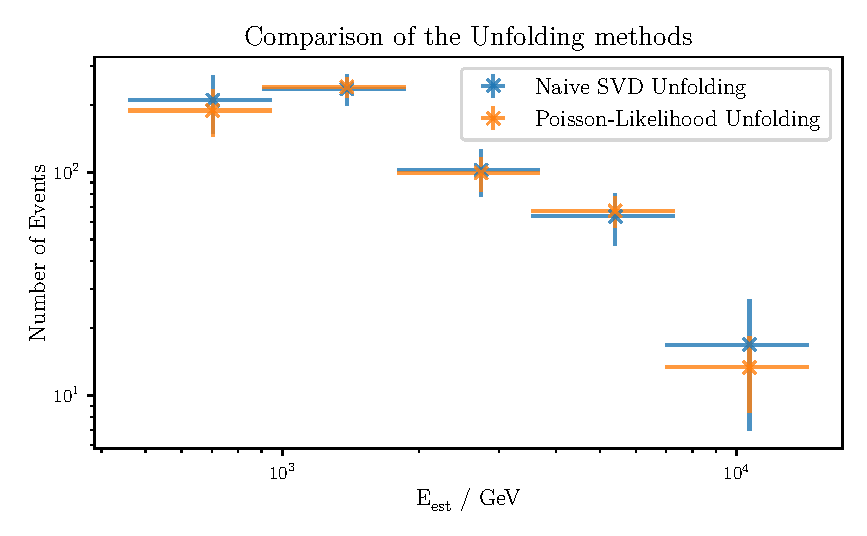
\includegraphics[width=\textwidth]{plots/Unfolding_compare.pdf}
  \caption{Comparison between both unfolding techniques.\label{fig:comp}}
\end{subfigure}
\end{figure}

The Poisson-likelihood method results in

\begin{align}
\hat{\symbf{f}} &=
\begin{pmatrix}
     188.75 \pm 40.98 \\
     241.08 \pm 15.70 \\
     99.47 \pm 17.74 \\
     67.21 \pm 13.92 \\
     13.37 \pm 6.24 \\
\end{pmatrix}
\end{align}

\subsection{Flux Calculation}
The flux is calculated with
\begin{equation}
  \phi_i = \frac{\hat{f}_i}{A_{\text{eff}, i} \Delta\symup{E}_i t_\text{obs}}\,.
  \label{eqn:flux}
\end{equation}
$\Delta\symup{E}_i$ is the width of the energy bin, $t_\text{obs}$ the duration of observation and $A_{\text{eff}, i}$ is calculated with
\begin{equation}
  A_{\text{eff}, i} = \frac{N_{\text{selec}, i}}{N_{\text{sim}, i}} \cdot A\,.
\end{equation}
Since only $70\%$ of the data is taken the effective detector area is divided by a factor of $0.7$.
The flux is calculated with both unfolding methods.
Figure \ref{fig:fluxBoth} shows the resulting fluxes which are very similar.

\begin{figure}[H]
  \centering
  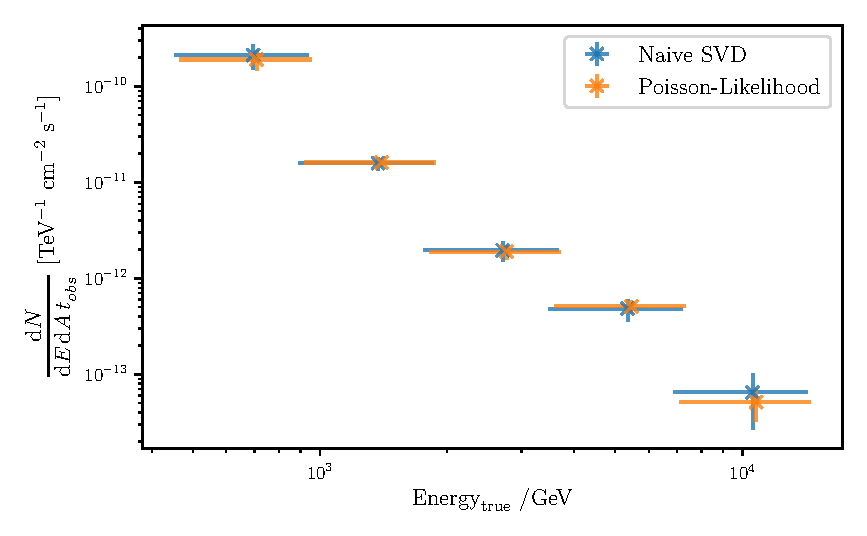
\includegraphics[width=0.8\textwidth]{plots/flux.pdf}
  \caption{flux calculation with naive SVD and Poisson-likelihood against true-energy.}
  \label{fig:fluxBoth}
\end{figure}

\subsection{Comparison with HEGRA and MAGIC}
The fitting function HEGRA and MAGIC used is defined as
\begin{equation}
  f(x, a, b, c, d) = a \left(\frac{x}{b}\right)^{\left(-c + d\cdot \ln\left(\frac{x}{b}\right)\right)}
\end{equation}

Table \ref{tab:vgl} shows the parameters of both measurements.

\begin{table}
  \centering
  \caption{Fitted values for the flux of the HEGRA \cite{HEGRA} and MAGIC \cite{MAGIC} experiment.}
  \label{tab:vgl}
  \sisetup{table-format=1.2}
  \begin{tabular}{l S @{${}\pm{}$} S S[table-format=1.0] S @{${}\pm{}$} S S @{${}\pm{}$} S}
    \toprule
    {Experiment} & \multicolumn{2}{c}{$a \mathbin{/} \si[per-mode=fraction]{\per\tera\electronvolt\per\centi\metre\squared} \times 10^{-11}$} & {$b \mathbin{/} \si{\tera\electronvolt}$} &  \multicolumn{2}{c}{$c$} &  \multicolumn{2}{c}{$d$} \\
    \midrule
    MAGIC & 3.23 & 0.03 & 1 & 2.47 & 0.01 & -0.24 & 0.01 \\
    HEGRA & 2.83 & 0.6 & 1 & 2.62 & 0.05 & 0 & 0 \\
    \bottomrule
  \end{tabular}
\end{table}

The results of this analysis is compatible with the results from MAGIC and HEGRA for energies bigger than $\SI{1}{TeV}$.
For lower energies our results are a bit off but still close enough to these results since the errorbar is almost reaching these results.


\begin{figure}[H]
  \centering
  \includegraphics[width=0.8\textwidth]{plots/flux_like.pdf}
  \caption{Comparison of our flux measurements with HEGRA and MAGIC.}
  \label{fig:fluxComp}
\end{figure}
